\section{Datasets and Monte Carlo Simulation}
\label{sec:DataSetAndMonteCarlo}

\subsection{LHC Dataset}
\label{subsec:Dataset}

The measurement uses the LHC collision data, named the ATLAS Run-$2$ dataset collected by the ATLAS experiment during its operation in $2015$, $2016$, $2017$, and $2018$. This dataset corresponds to proton-proton collisions at the center-of-mass energy of $\sqrt{s} = 13$ TeV and total integrated luminosity of $139 \pm 2.4$ fb$^{-1}$ measured by the LUCID-2 detector \cite{ATLASLuminosityDetector}\cite{ATLASRun2IntegratedLumi}. The uncertainty on the integrated luminosity is obtained by combining the measurements of LHC runs each year. Each data-taking run period is further divided into sub-periods of one to three weeks that vary in beam and detector conditions. The dataset used in physics analyses is required to satisfy a series of data quality checks discussed in detail in Ref \cite{ATLASRun2DataTaking}. The data passing these requirements collectively form a Good Run List (GRL) consisting of several luminosity blocks (LB). Figure \ref{fig:InstLuminosity} shows the total integrated luminosity delivered by LHC in the green distribution, recorded by the ATLAS experiment in the yellow distribution and part of the GRL in the blue distribution. The plateaus correspond to the end-of-year shutdowns of LHC, and the slopes correspond to the increasing instantaneous luminosity in different data-taking periods. 

\begin{figure}
\centering
\includegraphics[width=.8\linewidth]{figures/AnalysisOverview/IntegratedLumiRun2.pdf}  
  \caption{Total integrated luminosity collected during data taking period in Run-$2$ \cite{ATLASRun2DataTaking}. }
\label{fig:InstLuminosity}
\end{figure}

% The measurement uses the following data samples from the GRL,
% \begin{itemize}
% \footnotesize
% \item{ { GoodRunsLists/data15\_13TeV/20170619/PHYS\_StandardGRL\_All\_Good\_25ns\_276262-284484\_OflLumi-13TeV-008.root}}
% \item{  {GoodRunsLists/data16\_13TeV/20180129/PHYS\_StandardGRL\_All\_Good\_25ns\_297730-311481\_OflLumi-13TeV-009.root}}
% \item{{ GoodRunsLists/data17\_13TeV/20180619/physics\_25ns\_Triggerno17e33prim.lumicalc.OflLumi-13TeV-010.root}}
% \item{{GoodRunsLists/data18\_13TeV/20180924/physics\_25ns\_Triggerno17e33prim.lumicalc.OflLumi-13TeV-001.root}}
% \end{itemize}

% \normalsize

\subsection{Monte Carlo Samples }
\label{subsec:MCSamples}

As briefly mentioned in Section \ref{sec:Pheno}, the $pp \rightarrow ZZ (\rightarrow 4\ell) jj$ events are simulated by MC generators incorporating the matrix element calculations for the hard-scatter $pp \rightarrow ZZ (\rightarrow 4\ell) jj$ production, the parton showering, hadronization, the effect of the underlying events, and pile-up. The generated events are then simulated to interact with the ATLAS material using the Geant4 simulation toolkit following the description in Ref \cite{GEANT4}. The energy deposits of the simulated events in the detectors are then digitized and reconstructed using a detector geometry corresponding to the data-taking period. Each physics process is simulated using different generation campaigns corresponding to the different conditions of Run-2 ATLAS data-taking periods. Figure \ref{fig:MCGenerationSchematic} shows a schematic overview of the MC generation.
\begin{figure}
\centering
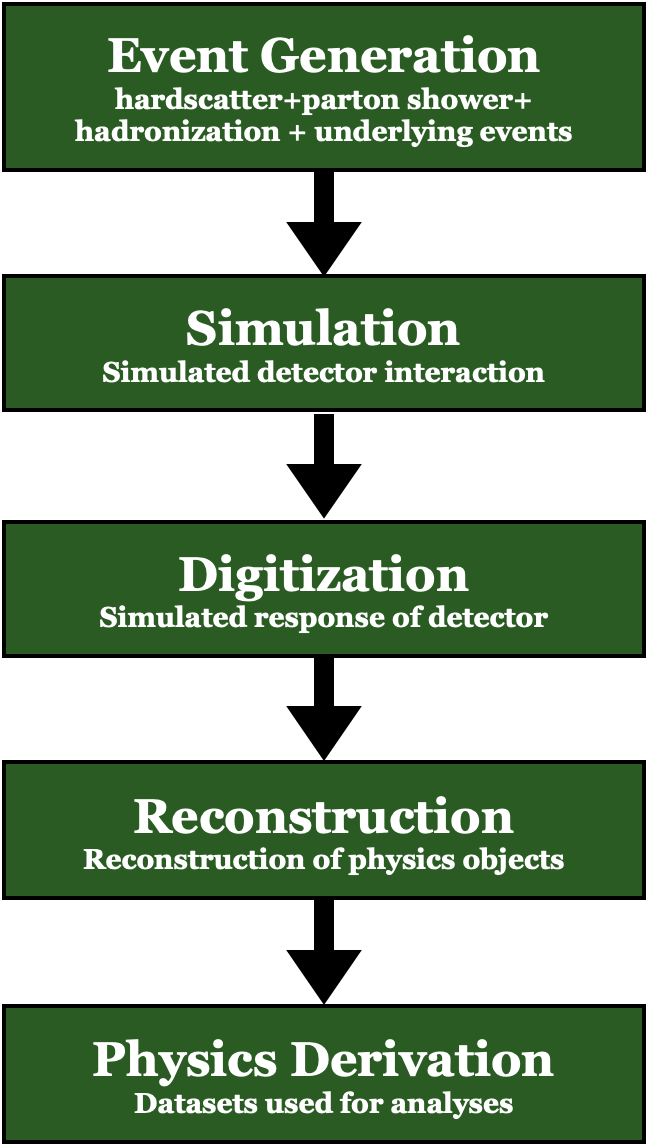
\includegraphics[width=.3\linewidth]{figures/AnalysisOverview/MCSchematic.png}  
  \caption{Various steps in MC sample generation.}
\label{fig:MCGenerationSchematic}
\end{figure}

\subsubsection{Signal Samples}
\label{subsubsec:SigSamples}
As discussed in Section \ref{sec:EWKPheno}, two types of interaction, QCD and EWK, give us $pp \rightarrow ZZ(\rightarrow 4 \ell) jj$ final state. The two types of QCD process, quark induced $qqZZ$ $[qq \rightarrow ZZ^*(\rightarrow 4 \ell) jj]$ and gluon induced $ggZZ$ $[gg \rightarrow ZZ^* (\rightarrow 4\ell) ]jj$ are simulated using the \textsc{Sherpa} $2.2.2$ MC generator. The parton initiated $qqZZ$ samples corresponding to Figure \ref{fig:ZZjjFeynmanDiag_QCD_qq} are generated with NLO accuracy in QCD up to one additional parton emission and LO accuracy for up to three additional partons emission. The loop-induced $ggZZ$ samples emerging at NNLO in $\alpha_{S}$ corresponding to Figure \ref{fig:ZZjjFeynmanDiag_QCD_gg} are generated using LO-accurate matrix elements for up to one additional parton emission \cite{EventGenWithSherpa}. The generator uses an NNPDF3.0NNLO PDF set evaluated using different measurements from several experiments, such as deep-inelastic inclusive cross-sections measurement from HERA-II, the combined charm data from HERA, jet production, vector boson rapidity and transverse momentum measurements from ATLAS, CMS and LHCb, total cross sections of top quark pair production from ATLAS and CMS and W+c data from CMS \cite{PDFForRunII}. Parton showering is done by \textsc{Sherpa}'s internal algorithm based on Catani–Seymour dipole factorization matrix element \cite{SherpaPS}. The matrix element calculations are matched and merged using the $ME+PS@NLO$ prescription \cite{PSMatching}. 

An alternative \textsc{MadGraph5} samples produced at NLO accuracy for up to one additional parton emission and LO accuracy for up to three additional parton emission \cite{MADGRAPHNLO} are also used in the measurement for the parton induced $qqZZ$ samples. The generator uses A14NNPDF23LO PDF set, and the ME is interfaced with \textsc{Pythia8} for parton showering, merging, and matching \cite{Pythia8}. 

The EWK production $qqZZjj$ $[qq \rightarrow ZZ^{*}(\rightarrow 4) \ell jj]$ is simulated using a \textsc{PowhegV2} generator using an MSTW2008 PDF set with NLO accuracy in QCD and interfaced with \textsc{Pythia8} for parton showering and hadronization \cite{PowhegV2}. An alternative sample at LO accuracy is also used in the measurement from \textsc{MadGraph5} with A14NNPDF23LO PDF set and \textsc{Pythia8} showering \cite{MADGRAPHNLO}. The \textsc{PowhegV2} NLO prediction of electroweak $qqZZjj$ does not contain the contribution from electroweak triboson $VZZ$ processes where two vector bosons decay leptonically and one decays hadronically. The contribution from these electroweak triboson processes is predicted using the {Sherpa} $2.2.2$ MC generator at LO accuracy for up to two additional parton emissions and added to the \textsc{PowhegV2} predictions. Table \ref{tab:SigMC} summarizes the signal MC used in the measurement. 

\begin{table}[!htb]
\footnotesize
\centering
\begin{tabular}{l l c c c }
\hline\hline
Process & Description & Generator  & PDF & Accuracy\\
\hline \hline
QCD $qqZZ$ &        &        &       &   \\
\multirow{2}{*}{ $q\bar{q} \rightarrow ZZ^{*}( \rightarrow 4\ell) jj$ } 
                    & \multirow{2}{*}{inclusive} & \textsc{Sherpa}$2.2.2$ & NNPDF3.0NNLO & \multirow{2}{*} {$0,1 j @NLO + 2,3 j @LO $} \\ 
        &  & \textsc{MadGraph} & A14NNPDF23LO & \\
        &       &        &       &   \\
\hline
QCD $ggZZ$ loop&        &        &       &   \\
 $gg \rightarrow ZZ^{*} (\rightarrow 4\ell) jj$ &  $m_{4 \ell } > 130$ GeV  & \textsc{Sherpa}$2.2.2$ & NNPDF3.0NNLO & $0,1 j @LO $ \\

&       &        &       &   \\

\hline 
EWK $qqZZjj$ &      &        &       &   \\
\multirow{2}{*}{ $q\bar{q} \rightarrow ZZ^{*}( \rightarrow 4\ell) jj$ } 
                    & \multirow{2}{*}{$m_{4\ell} > 130$ GeV } & \textsc{PowhegV2} & MSTW2008 &  $\ge 2 j$ (EWK) @ NLO QCD \\ 
        &   & \textsc{MadGraph} & A14NNPDF23LO & $\ge 2 j$ (EWK) @LO \\
        &       &        &       &   \\
\hline 
EWK $VZZ$ & & & & \\
$q\bar{q} \rightarrow VZZ^{*} \rightarrow 4\ell jj$ &       &   \textsc{Sherpa}$2.2.2$   &  NNPDF3.0NNLO     & $1,2j @LO$    \\
\hline\hline

\end{tabular}
\normalsize
\caption{List of signal MC samples used in the analysis. Each process consists of three different generation campaigns corresponding to the data-taking conditions of the ATLAS Run2 data-taking periods.\\ \label{tab:SigMC}}
\end{table}

\subsubsection{Background Samples}
\label{subsubsec:BkgSamples}

In addition to the QCD and EWK production discussed above, two other processes, triboson ($WWZ, ~WZZ, ~ZZZ$) and $Z$-bosons production in association with top quark pair ($t\bar{t}Z$), also contributes to the $ZZ (\rightarrow 4\ell) jj$ final state. The triboson processes are modeled with \textsc{Sherpa}$2.2.2$ generator at NLO accuracy in QCD for zero or one additional parton emissions and LO accuracy for up to two additional parton emissions. The triboson samples only include the fully leptonic decays of the vector bosons. Therefore, there is no overlap between the background triboson and the signal EWK $qqZZjj$ samples. The $t\bar{t}Z$ processes are modeled by \textsc{Sherpa}$2.2.0$ generator at LO accuracy with up to one additional parton emission using the MEPS@LO set-up \cite{Sherpa220}. The same algorithms as in the QCD $qqZZ$ sample generation are used for parton showering, matching, and merging. The MC simulation of the triboson and $t\bar{t}Z$ samples are subtracted directly from the data. Table \ref{tab:BkgMC} summarizes the details of these samples. 

\begin{table}[!htb]
\footnotesize
\centering
\begin{tabular}{l l c c c }
\hline\hline
Process & Description & Generator  & PDF & Accuracy\\
\hline \hline
 &      &        &       &   \\
 $pp \rightarrow W^{(*)}W^{(*)}Z^{(*)} \rightarrow 4\ell 2\nu $  & \multirow{3}{*}{inclusive} & \textsc{Sherpa}$2.2.2$ & \multirow{3}{*}{NNPDF3.0NNLO} & \multirow{3}{*}{$0,1 j @NLO + 2 j @LO $} \\ 
 
$pp \rightarrow W^{(*)}Z^{(*)}Z^{(*)} \rightarrow 5\ell 1\nu$  &  & \textsc{Sherpa}$2.2.2$ &   &  \\ 
$pp \rightarrow Z^{(*)} Z^{(*)} Z^{(*)} \rightarrow 6\ell $ &  & \textsc{Sherpa}$2.2.2$ &  &  \\ 
        
\hline 
&       &        &       &   \\
$pp \rightarrow t\bar{t}+Z(\rightarrow 2\ell)$ & $m_{ll} > 5$ GeV & \textsc{Sherpa}$2.2.0$ & NNPDF3.0NNLO & LO \\

\hline\hline
\end{tabular}
\normalsize
\caption{List of background MC samples used in the analysis. Each process consists of three different generation campaigns corresponding to the data-taking conditions of the ATLAS Run2 data-taking periods.\\ \label{tab:BkgMC}}
\end{table}

\subsubsection{Samples for Non-prompt Background}
\label{subsubsec:FakeBkgSamples}
In addition to the triboson and $t\bar{t}$Z samples, the analysis has additional backgrounds coming from events with one or more non-prompt or fake leptons. These non-prompt backgrounds are estimated using a data-driven method discussed in detail in Section \ref{subsec:FakeBackground}. MC samples are used to develop and validate the data-driven non-prompt background estimation procedure. Three sources of events could contribute as a source for non-prompt background events. The first type of events is from a Z-boson production in association with jets $pp \rightarrow Z^{(*)} \rightarrow 2\ell +jets$, which is simulated for both three or more leptons using \textsc{Sherpa}$2.2.1$. The subdominant process is events from $t\bar{t}\rightarrow 2\ell$ production in which both top quarks decay semileptonically, which is simulated with
\textsc{Powheg+Pythia8} and uses the A14NNPDF23LO PDF set \cite{PowhegPythia}. The third type of non-prompt backgrounds arises from the WZ production in which both bosons decay leptonically $pp \rightarrow WZ \rightarrow 2 \ell 1\nu $ and is simulated using \textsc{Sherpa}$2.2.2$. Table \ref{tab:FakeBkgMC} summarizes the different processes and MC generators used in various studies related to the data-driven fake factor method to estimate the non-prompt background.

\begin{table}[!htb]
\footnotesize
\centering
\begin{tabular}{l l c c c }
\hline\hline
Process & Description & Generator  & PDF & Accuracy\\
\hline \hline
 &      &        &       &   \\
 $pp \rightarrow Z^{(*)} \rightarrow 2e+jets $  & \multirow{3}{*}{inclusive} & \multirow{3}{*}{\textsc{Sherpa}$2.2.2$} & \multirow{3}{*}{NNPDF3.0NNLO} & \multirow{3}{*}{$NLO+2j,LO+4j $} \\ 
 
$pp \rightarrow Z^{(*)} \rightarrow 2\mu +jets $  &  &  &   &  \\ 
$pp \rightarrow Z^{(*)} \rightarrow 2\tau +jets $ &  &  &  &  \\ 
        
\hline 
&       &        &       &   \\
$pp \rightarrow t\bar{t} \rightarrow 2\ell $ & inclusive & \textsc{Powheg+Pythia8} & A14NNPDF23LO & LO \\
\hline 
&       &        &       &   \\
$pp \rightarrow WZ \rightarrow 2 \ell 1\nu $ & inclusive & \textsc{Sherpa}$2.2.2$ & NNPDF3.0NNLO & $NLO + 1j, LO+3j $\\
\hline\hline

\end{tabular}
\normalsize
\caption{List of MC samples used in the estimation and validation of the data-driven non-prompt background estimation.\\ \label{tab:FakeBkgMC}}
\end{table}

\subsection{Event Weights}
\label{subsec:EventWt}

The raw predictions from the MC generators are completely unscaled and cannot be compared to the data recorded by the detector directly. Each event generated by the MC needs to be scaled based on the cross-section of a given process normalized to the total sum of all the weights from events generated and multiplied by the integrated luminosity of the data-taking period. As shown by Figure \ref{fig:PileupDiffRuns}, the pile-up distribution is different for the different data-taking periods. The MC-generated events are modified to correctly simulate the effect of pile-up distribution imitating that of the data. Additionally, a set of measurement-related corrections are included in the event weight. These corrections, named \textit{ scaled factors (SF)}, correct the reconstruction, identification, isolation, and trigger efficiencies in the MC to match that of measured data. The total event weight for MC generated event is a product of the normalized generator weight scaled to match the pile-up profile and all scale factors.

\begin{figure}
\centering
\includegraphics[width=.8\linewidth]{figures/AnalysisOverview/mu_ProfileRun2.pdf}
\caption{Pile-up distributions in different Run-2 data-taking period.\label{fig:PileupDiffRuns} \cite{ATLASRun2DataTaking}}
\end{figure}
